\begin{center}
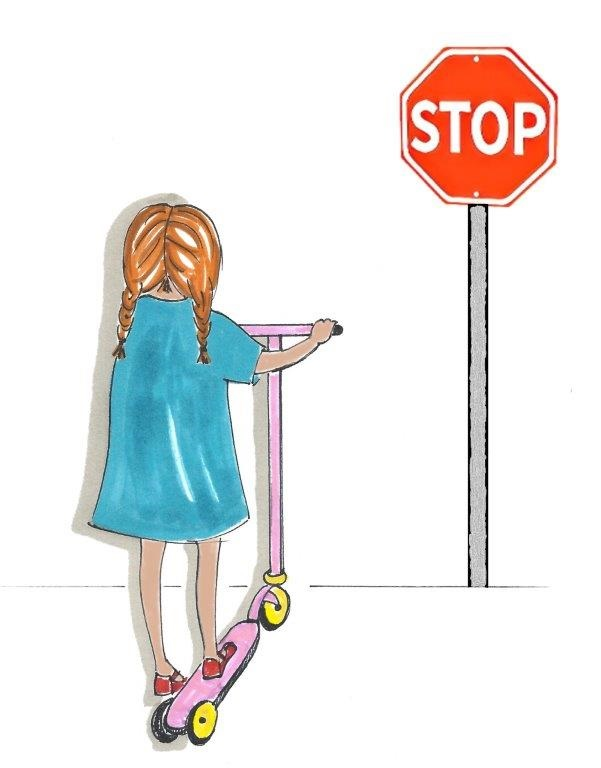
\includegraphics[width=0.6\textwidth]{content/3/chapter6/images/22.png}\\
Cippi stops in front of the stop sign
\end{center}

The additional functionality of the cooperative interruption thread is based on the std::stop\_token, the std::stop\_callback, and the std::stop\_source commands.

First, why it is not a good idea to kill a thread?

\begin{tcolorbox}[breakable,enhanced jigsaw,colback=red!5!white,colframe=red!75!black,title={Killing a Thread is Dangerous}]
	
Killing a thread is dangerous because you don’t know the state of the thread. Here are two possible malicious outcomes.

\begin{itemize}
\item 
The thread is only half-done with its job. Consequently, you don’t know the state of its job and, hence, the state of your program. You end with undefined behavior, and all bets are off

\item 
The thread may be in a critical section and having locked a mutex. Killing a thread while it locks a mutex ends with a high probability in a deadlock.
\end{itemize}
\end{tcolorbox}

\subsubsubsection{6.5.1\hspace{0.2cm} std::stop\_token, std::stop\_callback, and std::stop\_source}

A std::stop\_token, a std::stop\_callback, or a std::stop\_source command allows a thread to asynchronously request an execution to stop or ask if an execution got a stop signal. The std::stop\_token can be passed to an operation and afterward be used to actively poll the token for a stop request or to register a callback via std::stop\_callback. The stop request is sent by a std::stop\_source. This signal affects all associated std::stop\_token. The three classes std::stop\_source, std::stop\_token, and std::stop\_callback share the ownership of an associated stop state. The calls request\_stop(), stop\_requested(), and stop\_possible() are atomic.

You can construct a std::stop\_source in two ways:

\hspace*{\fill} \\ %插入空行
\noindent
Constructors of std::stop\_source
\begin{lstlisting}[style=styleCXX]
stop_source();
explicit stop_source(std::nostopstate_t) noexcept;
\end{lstlisting}

The default constructor (line 1) constructs a std::stop\_source with a new stop state. The constructor taking std::nostopstate\_t (line 2) constructs an empty std::stop\_source without associated stop state.

The component std::stop\_source src provides the following member functions for handling stop requests.

\begin{center}
Member functions of std::stop\_source src
\end{center}

\begin{table}[H]
\centering
\begin{tabular}{ll}
\textbf{Member function}       & \textbf{Description}                                                                   \\ \hline
src.get\_token() &
\begin{tabular}[c]{@{}l@{}}If stop\_possible(), returns a stop\_token for the associated stop state.\\ Otherwise, returns a default-constructed (empty) stop\_token.\end{tabular} \\
src.stop\_possible()  & true if src can be requested to stop.                                         \\
src.stop\_requested() & true if stop\_possible() and request\_stop() was called by one of the owners. \\
src.request\_stop() &
\begin{tabular}[c]{@{}l@{}}Calls a stop request if stop\_possible() and !stop\_requested(). Otherwise, the\\ call has no effect.\end{tabular}
\end{tabular}
\end{table}

src.stop\_possible() means that src has an associated stop state. src.stop\_requested() returns true when src has an associated stop state and was not asked to stop earlier. src.request\_stop() is successful and returns true if src has an associated stop state and it was not requested to stop before.

The call src.get\_token() returns the stop token stoken. Thanks to stoken you can check if a stop request has been made or can be made for its associated stop source src. The stop token stoken observes the stop source src.

\begin{center}
Member functions of std::stop\_token stoken
\end{center}

\begin{table}[H]
\centering
\begin{tabular}{ll}
\textbf{Member function} & \textbf{Description}                                                                                                                   \\ \hline
stoken.stop\_possible()  & Returns true if stoken has an associated stop state.                                                                                   \\
stoken.stop\_requested() & \begin{tabular}[c]{@{}l@{}}true if request\_stop() was called on the associated std::stop\_source src,\\ otherwise false.\end{tabular}
\end{tabular}
\end{table}

A default-constructed token that has no associated stop state. stoken.stop\_possible also returns true if the stop request has already been made. stoken.stop\_requested() returns true when the stop token has an associated stop state and has already received a stop request.

If the std::stop\_token should be temporarily disabled, you can replace it with a default-constructed token. A default-constructed token has no associated stop-state. The following code snippet shows how to disable and enable a thread’s capability to accept stop requests.

\hspace*{\fill} \\ %插入空行
\noindent
Temporarily disable a stop token
\begin{lstlisting}[style=styleCXX]
std::jthread jthr([](std::stop_token stoken) {
	...
	std::stop_token interruptDisabled;
	std::swap(stoken, interruptDisabled);
	...
	std::swap(stoken, interruptDisabled);
	...
}
\end{lstlisting}

std::stop\_token interruptDisabled has no associated stop state. This means, the thread jthr can accept stop requests in all lines except 4 and 5.

The next example shows the use of callbacks.

\hspace*{\fill} \\ %插入空行
\noindent
Use of callbacks
\begin{lstlisting}[style=styleCXX]
// invokeCallback.cpp

#include <atomic>
#include <chrono>
#include <iostream>
#include <thread>
#include <vector>

using namespace std::literals;

auto func = [](std::stop_token stoken) {
		std::atomic<int> counter{0};
		auto thread_id = std::this_thread::get_id();
		std::stop_callback callBack(stoken, [&counter, thread_id] {
			std::cout << "Thread id: " << thread_id
					  << "; counter: " << counter << '\n';
		});
		while (counter < 10) {
			std::this_thread::sleep_for(0.2s);
			++counter;
		}
	};

int main() {

	std::cout << '\n';
	
	std::vector<std::jthread> vecThreads(10);
	for(auto& thr: vecThreads) thr = std::jthread(func);
	
	std::this_thread::sleep_for(1s);
	
	for(auto& thr: vecThreads) thr.request_stop();
	
	std::cout << '\n';

}
\end{lstlisting}

Each of the ten threads invokes the lambda function func (lines 11 - 22). The callback in lines 14 - 17 displays the thread id and the counter. Due to the 1-second sleeping of the main thread and the sleeping of the child threads, the counter is four when the callbacks are invoked. The call thr.request\_stop() triggers the callback on each thread.

\begin{center}
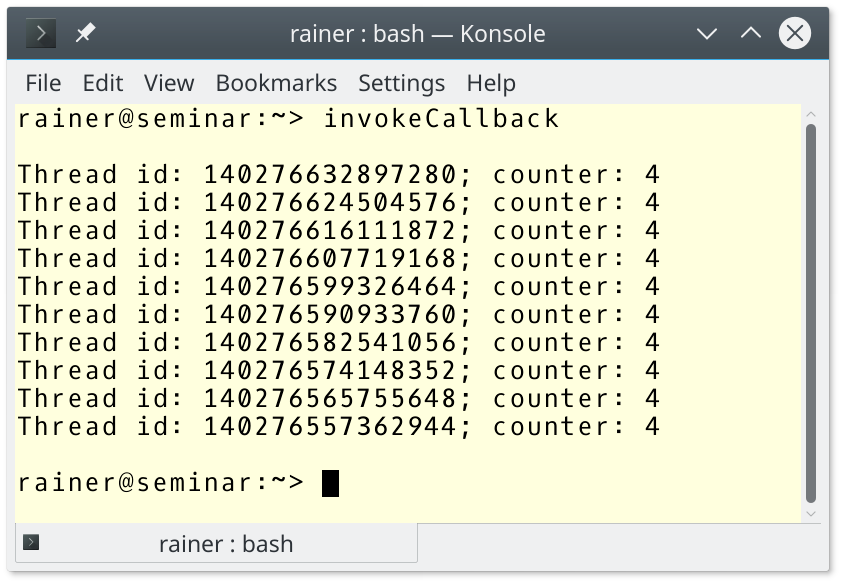
\includegraphics[width=0.8\textwidth]{content/3/chapter6/images/23.png}\\
Use of callbacks
\end{center}


\hspace*{\fill} \\ %插入空行
\noindent
\textbf{6.5.1.1\hspace{0.2cm} Joining Threads}

A std::jthread is a std::thread with the additional functionality to signal an interrupt and to automatically join(). To support this functionality it has a std::stop\_token.

\begin{center}
The member functions of std::jthread jthr for stop-token handling
\end{center}

\begin{table}[H]
\centering
\begin{tabular}{ll}
\textbf{Member Function}   & \textbf{Description}                                        \\ \hline
t.get\_stop\_source() & Returns a std::stop\_source object associated with the shared stop state. \\
t.get\_stop\_token()  & Returns a std::stop\_token object associated with the shared stop state.  \\
t.request\_stop() & Requests execution stop via the shared stop state.
\end{tabular}
\end{table}

\hspace*{\fill} \\ %插入空行
\noindent
\textbf{6.5.1.2\hspace{0.2cm} New wait Overloads for the condition\_variable\_any}

The three wait variations to wait, wait\_for, and wait\_until of the std::condition\_variable\_any get new overloads. They take a std::stop\_token.

\hspace*{\fill} \\ %插入空行
\noindent
Three new wait overloads
\begin{lstlisting}[style=styleCXX]
template <class Predicate>
bool wait(Lock& lock,
		stop_token stoken,
		Predicate pred);

template <class Rep, class Period, class Predicate>
bool wait_for(Lock& lock,
			stop_token stoken,
			const chrono::duration<Rep, Period>& rel_time,
			Predicate pred);

template <class Clock, class Duration, class Predicate>
bool wait_until(Lock& lock,
			stop_token stoken,
			const chrono::time_point<Clock, Duration>& abs_time,
			Predicate pred);
\end{lstlisting}

These new overloads need a predicate. The presented versions ensure that the threads be notified if a stop request for the passed std::stop\_token stoken is signaled. They return a boolean which indicates whether the predicate evaluates to true. This returned boolean is independent of whether a stop was requested or whether the timeout was triggered. The three overloads are equivalent to the following expressions:

\hspace*{\fill} \\ %插入空行
\noindent
Equivalent expression for the three overloads
\begin{lstlisting}[style=styleCXX]
// wait in lines 1 - 4
while (!stoken.stop_requested()) {
	if (pred()) return true;
	wait(lock);
}
return pred();

// wait_for in lines 6 - 10
return wait_until(lock,
					std::move(stoken),
					chrono::steady_clock::now() + rel_time,
					std::move(pred)
					);

// wait_until in lines 12 - 16
while (!stoken.stop_requested()) {
	if (pred()) return true;
	if (wait_until(lock, timeout_time) == std::cv_status::timeout) return pred();
}
return pred();
\end{lstlisting}

After the wait calls, you can check if a stop request happened.

\hspace*{\fill} \\ %插入空行
\noindent
Handle interrupts with wait
\begin{lstlisting}[style=styleCXX]
cv.wait(lock, stoken, predicate);
if (stoken.stop_requested()){
	// interrupt occurred
}
\end{lstlisting}

The following example shows the use of a condition variable with a stop request.

\hspace*{\fill} \\ %插入空行
\noindent
Use of condition variable with a stop request
\begin{lstlisting}[style=styleCXX]
// conditionVariableAny.cpp

#include <condition_variable>
#include <thread>
#include <iostream>
#include <chrono>
#include <mutex>
#include <thread>

using namespace std::literals;

std::mutex mut;
std::condition_variable_any condVar;

bool dataReady;

void receiver(std::stop_token stopToken) {

	std::cout << "Waiting" << '\n';
	
	std::unique_lock<std::mutex> lck(mut);
	bool ret = condVar.wait(lck, stopToken, []{return dataReady;});
	if (ret){
		std::cout << "Notification received: " << '\n';
	}
	else{
		std::cout << "Stop request received" << '\n';
	}
}

void sender() {

	std::this_thread::sleep_for(5ms);
	{
		std::lock_guard<std::mutex> lck(mut);
		dataReady = true;
		std::cout << "Send notification" << '\n';
	}
	condVar.notify_one();

}

int main(){

	std::cout << '\n';
	
	std::jthread t1(receiver);
	std::jthread t2(sender);
	
	t1.request_stop();
	
	t1.join();
	t2.join();
	
	std::cout << '\n';

}
\end{lstlisting}

The receiver thread (lines 17 - 29) is waiting for the notification of the sender thread (lines 31 - 41). Before the sender thread sends its notification in line 39, the main thread triggered a stop request in line 50. The output of the program shows that the stop request happened before the notification.

\begin{tcblisting}{breakable,commandshell={}}
Waiting
Stop request received
Send notification
\end{tcblisting}

\begin{center}
Sending a stop request to a condition variable
\end{center}

\begin{tcolorbox}[breakable,enhanced jigsaw,colback=mygreen!5!white,colframe=mygreen!75!black,title={Distilled Information}]
	
\begin{itemize}
\item 
Thanks to std::stop\_token, the std::stop\_source, and the std::stop\_callback, threads and condition variables can be cooperatively interrupted. Cooperative interruption means that the thread gets a stop request that it can accept or ignore.

\item 
The std::stop\_token can be passed to an operation and afterward be used to poll the token for a stop request actively or register a callback via std::stop\_callback.

\item 
Additionally to a std::jthread, std::condition\_variable\_any can also accept a stop request.
\end{itemize}
	
\end{tcolorbox}



















